\documentclass[11pt,a4paper]{article}
\usepackage[margin=2.2cm,headheight=14pt]{geometry}
\usepackage[T1]{fontenc}
\usepackage[utf8]{inputenc}
\usepackage{lmodern}
\usepackage{xcolor,graphicx,amsmath,amssymb,booktabs,array,longtable,listings}
\usepackage{tcolorbox,caption,tikz,pgfplots,microtype,enumitem,fancyhdr}
\usepackage{seqsplit,placeins}
\usepackage[colorlinks=true]{hyperref}
\pgfplotsset{compat=1.18}
\usetikzlibrary{arrows.meta,positioning,shapes.geometric}
\definecolor{cInput}{HTML}{527D83} % supplied input and measured input distributions
\definecolor{cProcess}{HTML}{35536B} % computation, method and comparison baseline
\definecolor{cResult}{HTML}{71839B} % computed output and measured outcomes
\definecolor{cAlert}{HTML}{D65A31} % sole high-saturation accent: point to notice
\definecolor{cNeutral}{HTML}{58616D} % axes, arrows and structural labels
\definecolor{cBg}{HTML}{F1F5F8} % quiet panel background
\hypersetup{linkcolor=cProcess,urlcolor=cProcess,citecolor=cProcess,pdftitle={Group 04: Parallel Case Studies},pdfauthor={Group 04 project report}}
\pagestyle{fancy}\fancyhf{}
\fancyhead[L]{\small Group 04 --- Parallel case studies}
\fancyhead[R]{\small\thepage}
\renewcommand{\headrulewidth}{0.3pt}
\setlength{\parindent}{0pt}
\setlength{\parskip}{4pt plus 1pt}
\setlength{\emergencystretch}{2em}
\setlength{\textfloatsep}{9pt plus 2pt minus 2pt}
\setlength{\intextsep}{8pt plus 2pt minus 2pt}
\captionsetup{font=small,labelfont=bf,skip=4pt}
\setlist{nosep,leftmargin=*}
\tcbset{colback=cProcess!5,colframe=cProcess,boxrule=.5pt,arc=1mm,left=2mm,right=2mm,top=1mm,bottom=1mm,fonttitle=\bfseries}
\lstset{basicstyle=\small\ttfamily,breaklines=true,backgroundcolor=\color{cBg},frame=single,rulecolor=\color{cNeutral}}
\newcommand{\TODO}[1]{\textcolor{cAlert}{[TODO: #1]}}
\newcommand{\term}[2]{\textbf{#1}: #2.}
\setcounter{tocdepth}{1}
\begin{document}
\begin{center}
{\LARGE\bfseries Group 04 --- Parallel case studies}\par
{\large CS3006 --- Assignment 3}\par
Fatima Malik (23L-0826) \quad Ibrahim Salman (23L-0723)\par
Measurements and analysis, 23 November 2026
\end{center}
\tableofcontents
\vspace{4pt}
\begin{tcolorbox}[title=Reading the visual language]
Muted teal identifies inputs, dark steel identifies computation, and slate identifies results.
The warm accent marks one finding to notice. Labels, marker shapes, dashes and hatching
preserve meaning without colour. Definitions explain terms at their first relevant section.
\end{tcolorbox}
\clearpage
\section*{Introduction}\addcontentsline{toc}{section}{Introduction}


\begin{tcolorbox}[title=Terms used in this section]\small \term{MPI}{Message Passing Interface, used by separate processes to exchange data} \term{rank}{an MPI process identifier} \term{OpenMP}{directives that divide work among threads sharing memory} \term{thread}{a worker within one process} \term{baseline}{the serial program used for comparison} \term{median}{the middle measured time} \term{SMT}{simultaneous multithreading, where one physical core runs multiple hardware threads} \term{WSL}{Windows Subsystem for Linux}\end{tcolorbox}

\textbf{CS3006 - Assignment 3}\newline{} Fatima Malik (23L-0826) and Ibrahim Salman (23L-0723)\newline{} Measurements and analysis, 23 November 2026.


\subsubsection*{Project scope}

Five C++17 serial/\allowbreak{}parallel implementations, correctness tests, three-repeat timings, plots and a six-slide presentation are included. Contribution status and the consolidated provenance disclosure are maintained in CONTRIBUTIONS.md.


\subsubsection*{Machine and toolchain}

AMD Ryzen 5 5500U: 6 physical cores, 12 logical processors. Host RAM: 7,866,085,376 bytes (7.33 GiB); WSL exposes approximately 3.5 GiB plus 1 GiB swap. Ubuntu WSL2, Linux 6.6.87.2; GCC 13.3.0 and Open MPI 4.1.6. All executables use -O3 -std=\allowbreak{}c++17 -Wall -Wextra -Wpedantic; OpenMP adds -fopenmp. This is a single-machine shared-memory MPI experiment, not a multi-node network experiment.


\subsubsection*{Measurement method}

Every reported point is the median of three independent process invocations. The raw TSV, source SHA-256 manifest, build log and environment dump are in results/\allowbreak{}. Generation and verification are outside timing except Monte Carlo, where generating random paths is part of the computation. MPI uses barriers around the timed region and reports maximum elapsed time across ranks. OpenMP uses OMP\_\allowbreak{}PROC\_\allowbreak{}BIND=\allowbreak{}close, OMP\_\allowbreak{}PLACES=\allowbreak{}cores, OMP\_\allowbreak{}DYNAMIC=\allowbreak{}false. MPI uses --bind-to core --map-by core. Workers are 1,2,4,6; only Monte Carlo additionally uses 8 workers (SMT). No MPI oversubscription is used.


S(p)=\allowbreak{}T\_\allowbreak{}serial/\allowbreak{}T\_\allowbreak{}parallel and E(p)=\allowbreak{}S(p)/\allowbreak{}p. The serial baseline is a separate executable, compiled with the same optimization level. Sort baselines recreate the same p-seeded shards. Runs execute sequentially; the agent cannot guarantee the Windows host was idle. WSL scheduling, background host activity, frequency changes and thermal state can affect results. Whiskers show the observed range, not confidence intervals. Interpret these as measurements of this session, and rerun on an idle machine for assessment.


\[S(p)=\frac{T_{\mathrm{serial}}}{T_{\mathrm{parallel}}},\qquad E(p)=\frac{S(p)}{p}.\] Speedup compares serial and parallel elapsed time; efficiency divides speedup by the worker count.

\begin{center}\small\setlength{\tabcolsep}{4pt}\renewcommand{\arraystretch}{1.12}

\begin{tabular}{@{}>{\raggedright\arraybackslash}p{\dimexpr 0.17021\linewidth-2.723pt\relax}>{\raggedright\arraybackslash}p{\dimexpr 0.44681\linewidth-7.149pt\relax}>{\raggedright\arraybackslash}p{\dimexpr 0.38298\linewidth-6.128pt\relax}@{}}\toprule

\textbf{Case} & \textbf{Model /\allowbreak{} decomposition} & \textbf{Final input}\\\midrule

Heat & MPI /\allowbreak{} 1-D rows and 2-D blocks & 1024\textsuperscript{2} and 4096\textsuperscript{2}; 500 steps\\

k-mers & OpenMP /\allowbreak{} window-start intervals & 100 million bases; k=\allowbreak{}8,12\\

Monte Carlo & OpenMP /\allowbreak{} fixed sample blocks & 100 million paths\\

PageRank & OpenMP /\allowbreak{} destination/\allowbreak{}source vertices & 65,\allowbreak{}536 vertices; 1 million edges\\

Sample sort & MPI /\allowbreak{} key buckets & 100 million 32-bit keys\\

\bottomrule\end{tabular}\end{center}

All 244 small-input comparisons passed before measurement: 49 heat, 60 k-mer, 9 Monte Carlo, 90 PageRank, 36 sort. Final six-worker tests bring the total to 255 comparisons, plus three known-value invariants. Deliberately incorrect variants are excluded. These tests do not prove correctness for every possible input.


\FloatBarrier

\section{Heat diffusion}

\begin{tcolorbox}[title=Terms used in this section]\small \term{stencil}{a repeated neighbor-based update rule} \term{halo}{copied neighbor cells around an owned block} \term{decomposition}{division of the grid among workers} \term{blocking}{waiting for an operation to complete before continuing} \term{nonblocking}{starting communication and completing it later} \term{Allreduce}{an MPI collective that combines values and returns the result to every rank} \term{convergence}{changes becoming sufficiently small}\end{tcolorbox}

\subsection{Implementation and scaling}

A two-grid explicit five-point stencil updates independent next-step cells from the old grid. Alpha=\allowbreak{}0.2; the top boundary is fixed at 100, other boundaries at zero. MPI fits spatial ownership and nearest-neighbor halos. Only interior cells are partitioned; uneven blocks are supported.


The ownership and data flow are summarized schematically in Figure~\ref{fig:flow1}.

\begin{figure}[htbp]\centering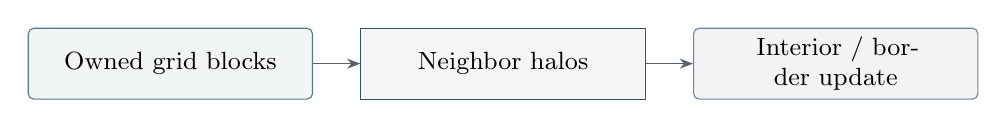
\begin{tikzpicture}[font=\small,>=Stealth,node distance=6mm, every node/.style={align=center,text width=3.4cm,minimum height=9mm,inner sep=3pt}]

\node[draw=cInput,fill=cInput!8,rounded corners=2pt] (a) {Owned grid blocks};

\node[draw=cProcess,fill=cProcess!6,right=of a] (b) {Neighbor halos};

\node[draw=cResult,fill=cResult!10,rounded corners=2pt,right=of b] (c) {Interior /\allowbreak{} border update};

\draw[->,cNeutral] (a)--(b);\draw[->,cNeutral] (b)--(c);\end{tikzpicture}

\caption{Schematic: ownership is separated from the communication or reduction that combines worker results.}\label{fig:flow1}\end{figure}

1-D: [row block 0] <halo rows> [row block 1] <halo rows> ...\newline{} 2-D: Cartesian block grid; each block exchanges north/\allowbreak{}south rows and east/\allowbreak{}west columns. Nonblocking: post halos -> compute strict interior -> wait -> compute border -> swap grids.


Blocking uses MPI\_\allowbreak{}Sendrecv; overlap uses Irecv/\allowbreak{}Isend and a vector datatype for columns. Every K steps and on the final step, Allreduce computes maximum change. There is no early stopping. The serial oracle checks every owned cell at absolute tolerance 1e-12, outside timing. The oracle is debug-only and replicated per rank.


The measured comparison is shown in Figure~\ref{fig:heat}.

\begin{figure}[htbp]\centering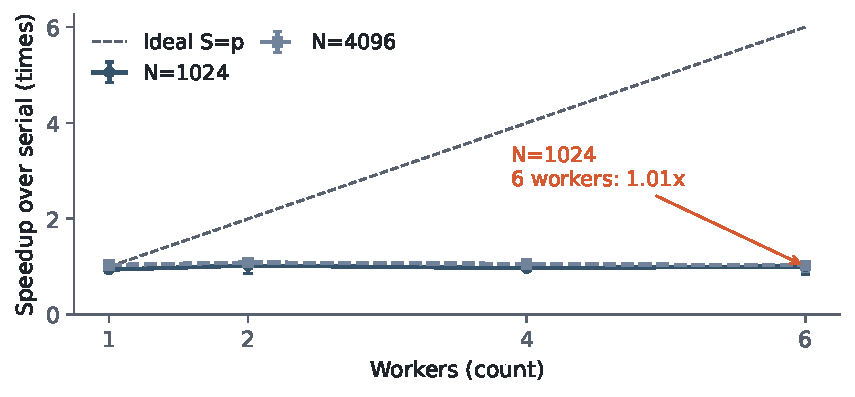
\includegraphics[width=0.9\textwidth]{figures/heat.pdf}

\caption{Heat speedup remains limited at both grid sizes; N=\allowbreak{}4096 reaches 1.03 times serial speed at six ranks. Both curves use 500 steps, 2-D overlap and K=\allowbreak{}50. Points are medians of three runs; whiskers span the minimum and maximum.}\label{fig:heat}\end{figure}

\begin{center}\small\setlength{\tabcolsep}{4pt}\renewcommand{\arraystretch}{1.12}

\begin{tabular}{@{}>{\raggedleft\arraybackslash}p{\dimexpr 0.07955\linewidth-2.545pt\relax}>{\raggedleft\arraybackslash}p{\dimexpr 0.23864\linewidth-7.636pt\relax}>{\raggedleft\arraybackslash}p{\dimexpr 0.25000\linewidth-8.000pt\relax}>{\raggedleft\arraybackslash}p{\dimexpr 0.20455\linewidth-6.545pt\relax}>{\raggedleft\arraybackslash}p{\dimexpr 0.22727\linewidth-7.273pt\relax}@{}}\toprule

\textbf{p} & \textbf{Serial (s)} & \textbf{Parallel (s)} & \textbf{S(p)} & \textbf{E(p)}\\\midrule

1 & 20.16 & 19.44 & 1.037 & 103.7\%\\

2 & 20.16 & 18.49 & 1.09 & 54.5\%\\

4 & 20.16 & 19.03 & 1.059 & 26.5\%\\

6 & 20.16 & 19.58 & 1.029 & 17.2\%\\

\bottomrule\end{tabular}\end{center}

Table: N=\allowbreak{}4096, 500 steps, 2-D overlap, K=\allowbreak{}50. N=\allowbreak{}1024 measurements and both input baselines are retained in summary.csv. Phase maxima are separately reduced and need not sum to maximum elapsed time.


\subsection{Critical analysis}

\subsubsection*{Surface-to-volume and overlap}

Let L=\allowbreak{}N-2. Work is approximately L\textsuperscript{2}/\allowbreak{}p cells/\allowbreak{}rank/\allowbreak{}step. Away from external boundaries, 1-D sends 2L halo values; a square 2-D layout sends 4L/\allowbreak{}sqrt(p). Receives add the same traffic again. Thus communication/\allowbreak{}work grows as 2p/\allowbreak{}L for 1-D and 4sqrt(p)/\allowbreak{}L for 2-D. For a rectangular a-by-b process grid, the interior send count is 2L/\allowbreak{}a+2L/\allowbreak{}b; physical-edge ranks communicate less. At p=\allowbreak{}1 there are no real neighbor transfers.


\begin{center}\small\setlength{\tabcolsep}{4pt}\renewcommand{\arraystretch}{1.12}

\begin{tabular}{@{}>{\raggedright\arraybackslash}p{\dimexpr 0.31915\linewidth-7.660pt\relax}>{\raggedleft\arraybackslash}p{\dimexpr 0.07447\linewidth-1.787pt\relax}>{\raggedleft\arraybackslash}p{\dimexpr 0.24468\linewidth-5.872pt\relax}>{\raggedleft\arraybackslash}p{\dimexpr 0.36170\linewidth-8.681pt\relax}@{}}\toprule

\textbf{Layout /\allowbreak{} exchange} & \textbf{K} & \textbf{Median (s)} & \textbf{Exposed exchange (s)}\\\midrule

1d /\allowbreak{} blocking & 1 & 1.254 & 0.05595\\

1d /\allowbreak{} blocking & 50 & 1.188 & 0.199\\

1d /\allowbreak{} overlap & 1 & 1.201 & 0.1654\\

1d /\allowbreak{} overlap & 50 & 1.185 & 0.1591\\

2d /\allowbreak{} blocking & 1 & 1.163 & 0.07664\\

2d /\allowbreak{} blocking & 50 & 1.169 & 0.2051\\

2d /\allowbreak{} overlap & 1 & 1.129 & 0.1648\\

2d /\allowbreak{} overlap & 50 & 1.156 & 0.207\\

\bottomrule\end{tabular}\end{center}

\textbf{At N=\allowbreak{}1024, p=\allowbreak{}4, K=\allowbreak{}50, overlap changes total time by 1.1\% relative to blocking (1.169 to 1.156 s).} This is the observed net effect, not a direct measure of transfer time hidden. Posting/\allowbreak{}wait timing excludes background transfer; shared-memory transport, progress, interior size and cache effects confound attribution. The formula predicts a lower asymptotic surface ratio for 2-D, but it does not guarantee a faster small single-node run.


For N=\allowbreak{}4096, efficiency first falls below 70\% at p=\allowbreak{}2. At six ranks the effective overhead T(p)-Tserial/\allowbreak{}p is 16.22 s. This residual includes memory-bandwidth contention and changed compute throughput, not just communication. Use Tcomp/\allowbreak{}p+Tcomm as an explanatory approximation, not a fitted network-only law. K=\allowbreak{}1 versus K=\allowbreak{}50 timings above expose the combined cost of more per-cell change work and more collectives; the change metric work is also conditional on K.


The measured comparison is shown in Figure~\ref{fig:weak}.

\begin{figure}[htbp]\centering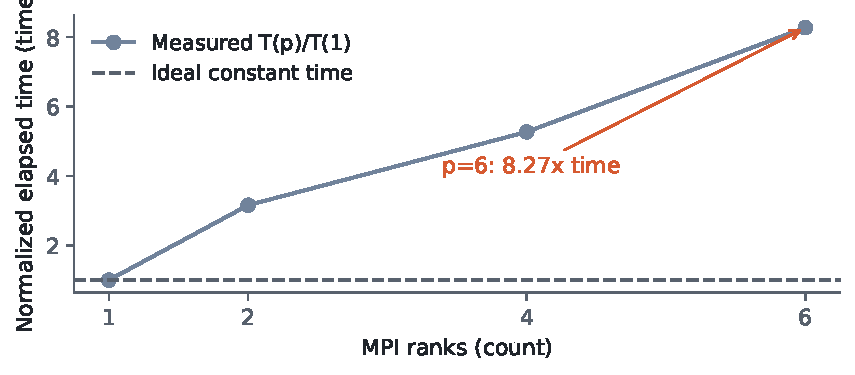
\includegraphics[width=0.9\textwidth]{figures/weak.pdf}

\caption{Heat weak-scaling time rises to 8.27 times the one-rank time despite approximately 512 squared interior cells per rank. Each point is the median of three runs.}\label{fig:weak}\end{figure}

Weak scaling uses N=\allowbreak{}2+round(512 sqrt(p)), 500 steps and K=\allowbreak{}50. Interior cells per rank stay near 262,144; rounding and rectangular process layouts change the exact surface. Ideal normalized time is one. The corresponding weak efficiency is T(1)/\allowbreak{}T(p), not serial strong-scaling speedup.


\FloatBarrier

\section{k-mer counting}

\begin{tcolorbox}[title=Terms used in this section]\small \term{k-mer}{a DNA substring of length k} \term{histogram}{a count for each possible substring} \term{atomic update}{an indivisible shared-counter update} \term{data race}{unsynchronized concurrent access with at least one write} \term{cache line}{the unit of data transferred through a processor cache} \term{false sharing}{workers modifying distinct values on one cache line, causing coherence traffic}\end{tcolorbox}

\subsection{Implementation and scaling}

Each DNA base occupies one byte and each k-mer uses a rolling two-bit index. Threads own disjoint ranges of window start positions, read k-1 bases past the range if necessary, and count boundary windows once. The serial baseline has O(L) rolling-window work.


The ownership and data flow are summarized schematically in Figure~\ref{fig:flow2}.

\begin{figure}[htbp]\centering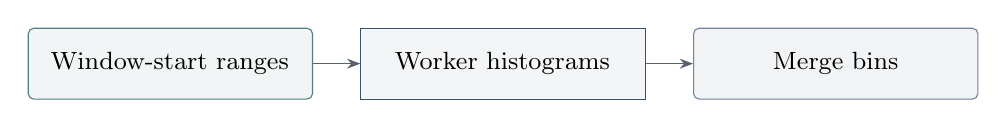
\begin{tikzpicture}[font=\small,>=Stealth,node distance=6mm, every node/.style={align=center,text width=3.4cm,minimum height=9mm,inner sep=3pt}]

\node[draw=cInput,fill=cInput!8,rounded corners=2pt] (a) {Window-start ranges};

\node[draw=cProcess,fill=cProcess!6,right=of a] (b) {Worker histograms};

\node[draw=cResult,fill=cResult!10,rounded corners=2pt,right=of b] (c) {Merge bins};

\draw[->,cNeutral] (a)--(b);\draw[->,cNeutral] (b)--(c);\end{tikzpicture}

\caption{Schematic: ownership is separated from the communication or reduction that combines worker results.}\label{fig:flow2}\end{figure}

DNA: A C G T ... -> disjoint window-start ranges -> worker histograms\newline{} A: shared increments (intentional race). B: shared atomic increments. C: private histograms -> merge by bin.


Fixed-seed SplitMix64 input is identical for every worker count. Integer verification compares every histogram bin and checks total L-k+1. Allocation/\allowbreak{}zeroing of the shared histogram and input generation are outside timing; private histogram allocation, initialization and merge are included. Verification is excluded. Counters are 64-bit.


The measured comparison is shown in Figure~\ref{fig:kmer}.

\begin{figure}[htbp]\centering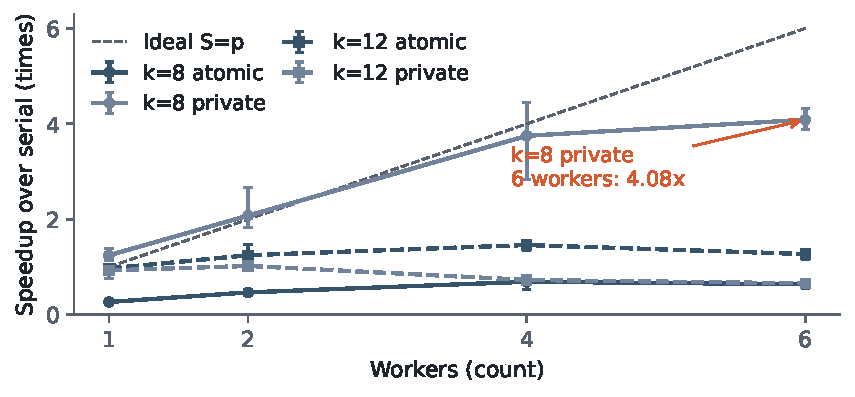
\includegraphics[width=0.9\textwidth]{figures/kmer.pdf}

\caption{The atomic and private histogram methods scale differently for k=\allowbreak{}8 and k=\allowbreak{}12. All runs count 100 million bases; circle/\allowbreak{}square markers distinguish k and solid/\allowbreak{}dashed lines remain readable in greyscale. Points are medians of three runs; whiskers span the minimum and maximum.}\label{fig:kmer}\end{figure}

\begin{center}\small\setlength{\tabcolsep}{4pt}\renewcommand{\arraystretch}{1.12}

\begin{tabular}{@{}>{\raggedleft\arraybackslash}p{\dimexpr 0.07955\linewidth-2.545pt\relax}>{\raggedleft\arraybackslash}p{\dimexpr 0.23864\linewidth-7.636pt\relax}>{\raggedleft\arraybackslash}p{\dimexpr 0.25000\linewidth-8.000pt\relax}>{\raggedleft\arraybackslash}p{\dimexpr 0.20455\linewidth-6.545pt\relax}>{\raggedleft\arraybackslash}p{\dimexpr 0.22727\linewidth-7.273pt\relax}@{}}\toprule

\textbf{p} & \textbf{Serial (s)} & \textbf{Parallel (s)} & \textbf{S(p)} & \textbf{E(p)}\\\midrule

1 & 0.1627 & 0.1307 & 1.245 & 124.5\%\\

2 & 0.1627 & 0.07841 & 2.076 & 103.8\%\\

4 & 0.1627 & 0.04342 & 3.748 & 93.7\%\\

6 & 0.1627 & 0.03984 & 4.085 & 68.1\%\\

\bottomrule\end{tabular}\end{center}

Table: k=\allowbreak{}8 private histograms. All four k/\allowbreak{}mode curves use L=\allowbreak{}100,000,000 and seed 42. Results for k=\allowbreak{}12 include substantially larger private allocation and merge costs; compare the measured totals rather than assuming the private method always wins.


\subsection{Critical analysis}

\textbf{Race:} in the first observed skewed-input demonstration, total=\allowbreak{}841371, expected=\allowbreak{}999993, and 159 bins differed. Two threads can read the same old count and each store old+1, losing an update. This is undefined behavior in C++; apparent agreement on another run would not make Version A correct.


\begin{center}\small\setlength{\tabcolsep}{4pt}\renewcommand{\arraystretch}{1.12}

\begin{tabular}{@{}>{\raggedleft\arraybackslash}p{\dimexpr 0.06383\linewidth-2.043pt\relax}>{\raggedleft\arraybackslash}p{\dimexpr 0.06383\linewidth-2.043pt\relax}>{\raggedleft\arraybackslash}p{\dimexpr 0.24468\linewidth-7.830pt\relax}>{\raggedleft\arraybackslash}p{\dimexpr 0.24468\linewidth-7.830pt\relax}>{\raggedleft\arraybackslash}p{\dimexpr 0.38298\linewidth-12.255pt\relax}@{}}\toprule

\textbf{k} & \textbf{p} & \textbf{Atomic (s)} & \textbf{Private (s)} & \textbf{Private memory}\\\midrule

8 & 1 & 0.6093 & 0.1307 & 0 MiB\\

8 & 2 & 0.3478 & 0.07841 & 1 MiB\\

8 & 4 & 0.2353 & 0.04342 & 2 MiB\\

8 & 6 & 0.2549 & 0.03984 & 3 MiB\\

12 & 1 & 2.265 & 2.361 & 128 MiB\\

12 & 2 & 1.761 & 2.146 & 256 MiB\\

12 & 4 & 1.502 & 3.014 & 512 MiB\\

12 & 6 & 1.73 & 3.34 & 768 MiB\\

\bottomrule\end{tabular}\end{center}

{\small\textbf{Rounding note.} The supplied table rounds memory to whole MiB. Its ``0 MiB entry represents 512 KiB after rounding, not a zero allocation.}

Private memory is 4\textasciicircum{}k * 8 * p bytes: 512 KiB/\allowbreak{}worker at k=\allowbreak{}8 and 128 MiB/\allowbreak{}worker at k=\allowbreak{}12. The six-core CPU has 512 KiB L2/\allowbreak{}core and a shared 4 MiB L3. k=\allowbreak{}8 can exploit locality but k=\allowbreak{}12 greatly exceeds cache, with extra zeroing and merge traffic. Atomic updates pay read-modify-write/\allowbreak{}coherence costs; private bins avoid contention but multiply memory and merge work. The table gives the actual crossover, including overhead rather than only the counting loop.


\begin{center}\small\setlength{\tabcolsep}{4pt}\renewcommand{\arraystretch}{1.12}

\begin{tabular}{@{}>{\raggedleft\arraybackslash}p{\dimexpr 0.07447\linewidth-1.787pt\relax}>{\raggedleft\arraybackslash}p{\dimexpr 0.27660\linewidth-6.638pt\relax}>{\raggedleft\arraybackslash}p{\dimexpr 0.32979\linewidth-7.915pt\relax}>{\raggedleft\arraybackslash}p{\dimexpr 0.31915\linewidth-7.660pt\relax}@{}}\toprule

\textbf{p} & \textbf{Packed (s)} & \textbf{64-byte padded (s)} & \textbf{Packed /\allowbreak{} padded}\\\midrule

1 & 0.03495 & 0.03647 & 0.9581\\

2 & 0.706 & 0.08578 & 8.23\\

4 & 1.726 & 0.09686 & 17.82\\

6 & 2.47 & 0.1143 & 21.62\\

\bottomrule\end{tabular}\end{center}

The counter microbenchmark performs 100 million volatile increments per worker. Separate counters share cache lines when packed; alignas(64) separates them under this CPU cache-line assumption. Each worker owns a distinct object, so this is false sharing rather than a data race. Padding ratios above are measured, not a guaranteed speedup; the short microbenchmark is sensitive to scheduling and CPU state.


Rolling scans read about one new sequence byte/\allowbreak{}window after each initial k-byte window. At p=\allowbreak{}6, k=\allowbreak{}8 private reaches 2.51e+03 million windows/\allowbreak{}s; k=\allowbreak{}12 private reaches 29.9. Histogram loads/\allowbreak{}stores, cache-line transfers, atomic coherence and merges dominate additional traffic. These input-read rates are not measured DRAM bandwidth. The finite cache and added private memory explain why additional workers can stop helping; hardware counters would be needed to separate bandwidth saturation from scheduling effects.


\FloatBarrier

\section{Monte Carlo}

\begin{tcolorbox}[title=Terms used in this section]\small \term{Monte Carlo}{estimation using pseudorandom samples} \term{variance}{how spread out values are around their average} \term{standard error}{estimated uncertainty in the sample mean} \term{Box--Muller}{a transform from uniform samples to normal samples} \term{closed form}{a direct mathematical formula} \term{reduction}{combining worker results} \term{Amdahl fraction}{the effective part of execution that does not benefit from more workers}\end{tcolorbox}

\subsection{Implementation and scaling}

European call pricing uses S0=\allowbreak{}100, strike=\allowbreak{}100, r=\allowbreak{}0.05, sigma=\allowbreak{}0.2 and T=\allowbreak{}1 year. Payoff is exp(-rT)*max(S\_\allowbreak{}T-K,0), with S\_\allowbreak{}T=\allowbreak{}100*exp(0.03+0.2Z). Box-Muller produces normal samples. Standard error is sqrt(sample variance/\allowbreak{}M), using M-1 degrees of freedom.


The ownership and data flow are summarized schematically in Figure~\ref{fig:flow3}.

\begin{figure}[htbp]\centering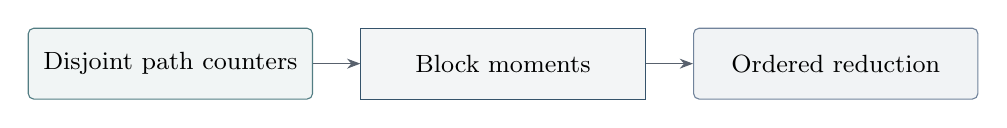
\begin{tikzpicture}[font=\small,>=Stealth,node distance=6mm, every node/.style={align=center,text width=3.4cm,minimum height=9mm,inner sep=3pt}]

\node[draw=cInput,fill=cInput!8,rounded corners=2pt] (a) {Disjoint path counters};

\node[draw=cProcess,fill=cProcess!6,right=of a] (b) {Block moments};

\node[draw=cResult,fill=cResult!10,rounded corners=2pt,right=of b] (c) {Ordered reduction};

\draw[->,cNeutral] (a)--(b);\draw[->,cNeutral] (b)--(c);\end{tikzpicture}

\caption{Schematic: ownership is separated from the communication or reduction that combines worker results.}\label{fig:flow3}\end{figure}

Global path indices -> disjoint counter ranges -> fixed 65,536-path blocks\newline{} Workers compute (payoff sum, squared-payoff sum) -> ordered block reduction -> price and standard error.


OpenMP is appropriate because paths are independent and communicate only final partial moments. Two unique counters per path are mapped through a SplitMix64 permutation, avoiding shared RNG state and duplicate stream assignments. This is a pseudorandom method, not a claim of mathematically independent random variables. Ordered block reduction in long double makes numerical output independent of scheduling and p on this toolchain. Both price and standard error are checked against serial with absolute tolerance 1e-12.


The measured comparison is shown in Figure~\ref{fig:mc}.

\begin{figure}[htbp]\centering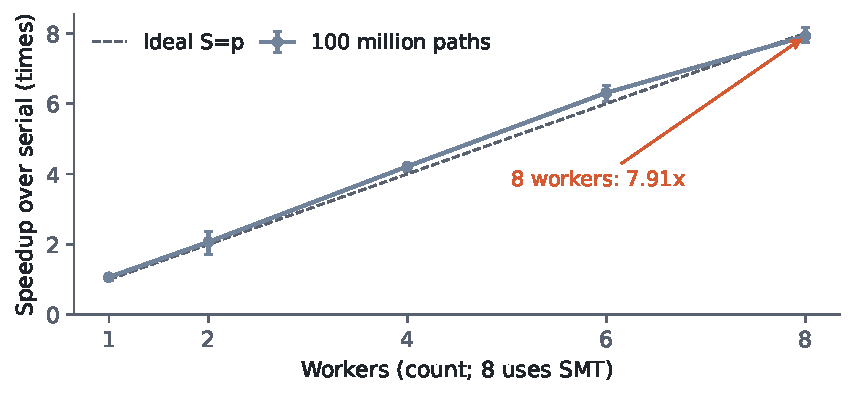
\includegraphics[width=0.9\textwidth]{figures/mc.pdf}

\caption{Monte Carlo reaches 6.31 times serial speed at six workers for 100 million paths. Eight workers use simultaneous multithreading on six physical cores. Points are medians of three runs; whiskers span the minimum and maximum.}\label{fig:mc}\end{figure}

\begin{center}\small\setlength{\tabcolsep}{4pt}\renewcommand{\arraystretch}{1.12}

\begin{tabular}{@{}>{\raggedleft\arraybackslash}p{\dimexpr 0.07955\linewidth-2.545pt\relax}>{\raggedleft\arraybackslash}p{\dimexpr 0.23864\linewidth-7.636pt\relax}>{\raggedleft\arraybackslash}p{\dimexpr 0.25000\linewidth-8.000pt\relax}>{\raggedleft\arraybackslash}p{\dimexpr 0.20455\linewidth-6.545pt\relax}>{\raggedleft\arraybackslash}p{\dimexpr 0.22727\linewidth-7.273pt\relax}@{}}\toprule

\textbf{p} & \textbf{Serial (s)} & \textbf{Parallel (s)} & \textbf{S(p)} & \textbf{E(p)}\\\midrule

1 & 10.34 & 9.687 & 1.068 & 106.8\%\\

2 & 10.34 & 5.003 & 2.067 & 103.4\%\\

4 & 10.34 & 2.454 & 4.214 & 105.4\%\\

6 & 10.34 & 1.64 & 6.307 & 105.1\%\\

\bottomrule\end{tabular}\end{center}

\textbf{For 100 million paths, price=\allowbreak{}10.45191667, standard error=\allowbreak{}0.00147211, analytic Black-Scholes=\allowbreak{}10.45058357, standardized deviation=\allowbreak{}0.906.} Statistical error is distinct from serial-equivalence error. Random path generation is included in computation timing.


\subsection{Critical analysis}

\subsubsection*{Why random stream ownership matters}

At p=\allowbreak{}8, good-stream price=\allowbreak{}10.45191667; intentional repeated-stream price=\allowbreak{}10.45327343. The bad version reports naive SE=\allowbreak{}0.00147226, but repeating 12.5 million unique paths eight times does not yield 100 million independent observations. An approximate corrected SE is sqrt(8) times larger: 0.00416418. Reusing the same worker seed corrupts the uncertainty estimate even when the price looks plausible. A locked shared generator would instead add serial contention; this implementation avoids both designs.


\subsubsection*{Accuracy per second and the fixed-time experiment}

\begin{center}\small\setlength{\tabcolsep}{4pt}\renewcommand{\arraystretch}{1.12}

\begin{tabular}{@{}>{\raggedleft\arraybackslash}p{\dimexpr 0.13830\linewidth-3.319pt\relax}>{\raggedleft\arraybackslash}p{\dimexpr 0.30851\linewidth-7.404pt\relax}>{\raggedleft\arraybackslash}p{\dimexpr 0.27660\linewidth-6.638pt\relax}>{\raggedleft\arraybackslash}p{\dimexpr 0.27660\linewidth-6.638pt\relax}@{}}\toprule

\textbf{Workers} & \textbf{Paths} & \textbf{Actual time (s)} & \textbf{Standard error}\\\midrule

1 & 123880466 & 13.56 & 0.001323\\

8 & 918147304 & 13.05 & 0.0004858\\

\bottomrule\end{tabular}\end{center}

Each workload was calibrated from measured throughput to a twelve-second target with at least 100 million paths, then run three times; actual times above disclose the mismatch. This is approximately fixed time, not a deadline-controlled sampler. The observed SE reduction factor is 2.72. Since SE is proportional to 1/\allowbreak{}sqrt(M), a throughput gain g yields about sqrt(g) more precision at fixed time, or 1/\allowbreak{}g of the time for a fixed target variance. Eight workers use SMT on six physical cores, so their gain cannot be read as eight-core scaling. Earlier three-second exploratory runs are retained separately in the raw data.


\subsubsection*{Amdahl estimate and limitations}

At p=\allowbreak{}6, speedup=\allowbreak{}6.307; the effective Amdahl fraction f=\allowbreak{}(1/\allowbreak{}S-1/\allowbreak{}p)/\allowbreak{}(1-1/\allowbreak{}p) is -0.009749. This is an effective fit from one point, not a measured proportion of serial instructions. Reduction, startup, shared execution resources, CPU turbo/\allowbreak{}thermal behavior, virtualization and host load can all enter the fitted fraction. A negative or >1 fit would signal a poor model rather than a physical fraction. This workload has little communication, but its observed scaling must be used rather than the assumption that it scales perfectly.


\subsubsection*{Reproducibility}

The spread in recorded good-stream prices across p=\allowbreak{}1,2,4,6,8 is 0. Fixed path indices select the same random values, each block keeps the same internal summation order, and the final reduction follows block order. A usual worker-seeded implementation changes sample assignments with p; an OpenMP floating-point reduction may also change the reduction tree. Because addition is not associative, such implementations can change the final low-order bits even for identical samples. Reproducibility here is within this compiler/\allowbreak{}platform, not a promise of bitwise cross-platform math-library behavior.


\FloatBarrier

\section{PageRank}

\begin{tcolorbox}[title=Terms used in this section]\small \term{CSR}{compressed sparse row storage: offsets plus adjacent vertex identifiers} \term{degree}{the number of incident edges in the specified direction} \term{dangling vertex}{a vertex with no outgoing edges} \term{pull}{each destination reads its incoming contributions} \term{push}{each source adds contributions to destinations} \term{chunk}{a group of iterations scheduled together} \term{L1 residual}{the sum of absolute rank changes} \term{R-MAT}{a recursive matrix method for generating an irregular graph}\end{tcolorbox}

\subsection{Implementation and scaling}

A fixed-seed R-MAT directed multigraph has 65,536 vertices and one million edges. Quadrant probabilities are (0.57,0.19,0.19,0.05); self-loops and duplicate edges remain. Incoming and outgoing CSR avoid per-edge object overhead. Damping is 0.85, L1 convergence tolerance 1e-10, and the safety cap is 500 iterations.


The ownership and data flow are summarized schematically in Figure~\ref{fig:flow4}.

\begin{figure}[htbp]\centering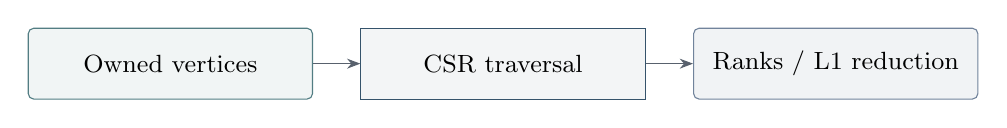
\begin{tikzpicture}[font=\small,>=Stealth,node distance=6mm, every node/.style={align=center,text width=3.4cm,minimum height=9mm,inner sep=3pt}]

\node[draw=cInput,fill=cInput!8,rounded corners=2pt] (a) {Owned vertices};

\node[draw=cProcess,fill=cProcess!6,right=of a] (b) {CSR traversal};

\node[draw=cResult,fill=cResult!10,rounded corners=2pt,right=of b] (c) {Ranks /\allowbreak{} L1 reduction};

\draw[->,cNeutral] (a)--(b);\draw[->,cNeutral] (b)--(c);\end{tikzpicture}

\caption{Schematic: ownership is separated from the communication or reduction that combines worker results.}\label{fig:flow4}\end{figure}

Pull: destination-owned CSR rows <- read in-neighbor contributions (no writes shared)\newline{} Push: source-owned CSR rows -> atomic contributions to destination ranks\newline{} All workers reduce dangling mass and L1 change each iteration.


Dangling vertices redistribute their mass uniformly. Each next rank begins with (1-d)/\allowbreak{}n+d*dangling/\allowbreak{}n. Serial is pull; parallel pull/\allowbreak{}push verify maximum error <=\allowbreak{}1e-9, L1 error <=\allowbreak{}1e-8, mass within 1e-8 of one, and convergence. Tests include a graph with zero edges. Graph/\allowbreak{}CSR creation is excluded; contribution preparation and all iteration overhead are included.


The measured comparison is shown in Figure~\ref{fig:pagerank}.

\begin{figure}[htbp]\centering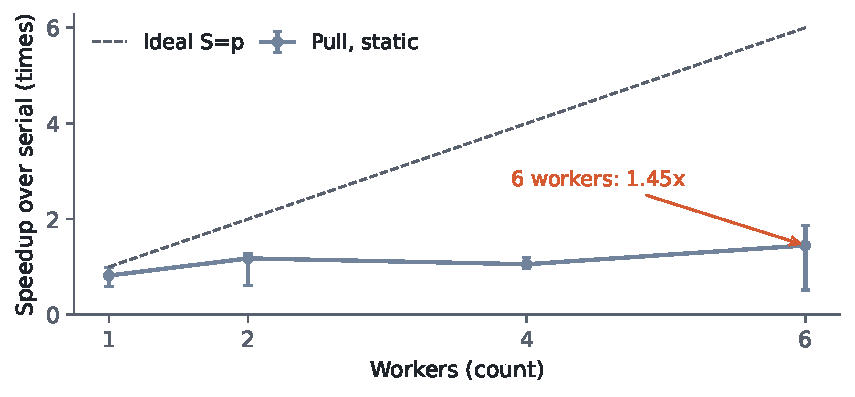
\includegraphics[width=0.9\textwidth]{figures/pagerank.pdf}

\caption{Contiguous static pull reaches 1.45 times serial speed at six workers for a one-million-edge graph; scheduling alternatives are compared separately. Points are medians of three runs; whiskers span the minimum and maximum.}\label{fig:pagerank}\end{figure}

\begin{center}\small\setlength{\tabcolsep}{4pt}\renewcommand{\arraystretch}{1.12}

\begin{tabular}{@{}>{\raggedleft\arraybackslash}p{\dimexpr 0.07955\linewidth-2.545pt\relax}>{\raggedleft\arraybackslash}p{\dimexpr 0.23864\linewidth-7.636pt\relax}>{\raggedleft\arraybackslash}p{\dimexpr 0.25000\linewidth-8.000pt\relax}>{\raggedleft\arraybackslash}p{\dimexpr 0.20455\linewidth-6.545pt\relax}>{\raggedleft\arraybackslash}p{\dimexpr 0.22727\linewidth-7.273pt\relax}@{}}\toprule

\textbf{p} & \textbf{Serial (s)} & \textbf{Parallel (s)} & \textbf{S(p)} & \textbf{E(p)}\\\midrule

1 & 0.04007 & 0.04895 & 0.8186 & 81.9\%\\

2 & 0.04007 & 0.03401 & 1.178 & 58.9\%\\

4 & 0.04007 & 0.03797 & 1.056 & 26.4\%\\

6 & 0.04007 & 0.02767 & 1.448 & 24.1\%\\

\bottomrule\end{tabular}\end{center}

The four-worker static pull run converged in 22 iterations with rank sum 0.999999999999. Static work-loop imbalance max/\allowbreak{}mean is 1.89. Timers stop before the final loop barrier; including barrier wait would hide the imbalance.


\subsection{Critical analysis}

The measured comparison is shown in Figure~\ref{fig:degrees}.

\begin{figure}[htbp]\centering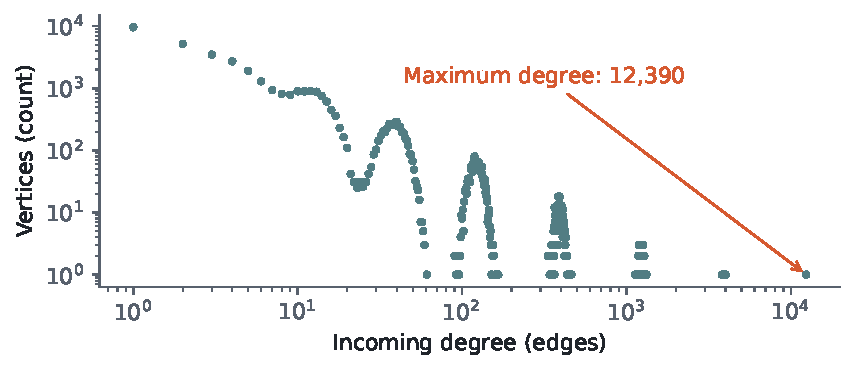
\includegraphics[width=0.9\textwidth]{figures/degrees.pdf}

\caption{The fixed-seed R-MAT graph has highly unequal incoming degrees. Zero-degree vertices remain in the solver but are excluded from these logarithmic axes.}\label{fig:degrees}\end{figure}

Equal vertex counts do not imply equal work: high-degree destinations require longer CSR scans. The degree plot shows the actual graph rather than assuming a perfect power law. Incoming degree zero is excluded from log axes, but the solver keeps all vertices. The imbalance ratio measures accumulated edge-loop time, including scheduler overhead and excluding final wait.


\begin{center}\small\setlength{\tabcolsep}{4pt}\renewcommand{\arraystretch}{1.12}

\begin{tabular}{@{}>{\raggedright\arraybackslash}p{\dimexpr 0.36170\linewidth-5.787pt\relax}>{\raggedleft\arraybackslash}p{\dimexpr 0.31915\linewidth-5.106pt\relax}>{\raggedleft\arraybackslash}p{\dimexpr 0.31915\linewidth-5.106pt\relax}@{}}\toprule

\textbf{Schedule /\allowbreak{} chunk} & \textbf{Pull seconds} & \textbf{Push seconds}\\\midrule

static /\allowbreak{} 1 & 0.03636 & 0.1311\\

static /\allowbreak{} 64 & 0.04311 & 0.1322\\

static /\allowbreak{} 256 & 0.03607 & 0.119\\

dynamic /\allowbreak{} 1 & 0.08489 & 0.1436\\

dynamic /\allowbreak{} 64 & 0.0165 & 0.1087\\

dynamic /\allowbreak{} 256 & 0.01528 & 0.09989\\

guided /\allowbreak{} 1 & 0.02264 & 0.1229\\

guided /\allowbreak{} 64 & 0.02166 & 0.1191\\

guided /\allowbreak{} 256 & 0.01988 & 0.1136\\

\bottomrule\end{tabular}\end{center}

\textbf{The fastest tested four-worker configuration is pull, dynamic chunk 256 at 0.01528 s.} Small dynamic chunks can improve work balance but require more scheduling operations; larger chunks amortize scheduling while leaving some imbalance. Static cyclic chunks redistribute concentrated degrees, while contiguous static creates a different ownership pattern. Results, not labels, decide the best setting.


At dynamic chunk 64, push/\allowbreak{}pull time ratio is 6.59 (0.1087/\allowbreak{}0.0165 s). Push includes random atomic destination writes and cache-line contention; pull uses random source reads and exclusive output writes. This ratio is a combined traversal/\allowbreak{}atomic cost comparison, not an isolated atomic latency measurement.


Best configuration throughput is 1.44e+03 million edges/\allowbreak{}s. A simple pull model counts 4-byte neighbor IDs plus 8-byte contribution reads per edge before reuse, giving an effective 17.3 GB/\allowbreak{}s, plus O(vertices) traffic. Contributions fit much better in cache than the entire edge structure, so effective traffic is not measured DRAM traffic. No independent memory-bandwidth ceiling was measured: proximity to that ceiling cannot be quantified honestly. The access pattern, schedule overhead and contention identify likely costs, but a STREAM/\allowbreak{}hardware-counter run would be needed for a roofline claim.


\FloatBarrier

\section{Sample sort}

\begin{tcolorbox}[title=Terms used in this section]\small \term{splitter}{a key value separating output buckets} \term{bucket}{the keys assigned to one destination rank} \term{oversampling}{collecting extra candidate splitters} \term{fingerprint}{a compact checksum used to detect likely data changes} \term{latency}{the fixed delay of a transfer} \term{bandwidth}{the amount of data transferred per second} \term{Alltoallv}{an MPI collective that exchanges different amounts of data between ranks}\end{tcolorbox}

\subsection{Implementation and scaling}

Each MPI rank owns an independently seeded shard of the 100-million-key input. Uniform keys are 32-bit values; skew sets approximately 90\% of keys to zero. Local sorting is followed by p-1 regular samples/\allowbreak{}rank, global quantile splitters, bucket partitioning, Alltoall counts, Alltoallv keys, then a final local sort.


The ownership and data flow are summarized schematically in Figure~\ref{fig:flow5}.

\begin{figure}[htbp]\centering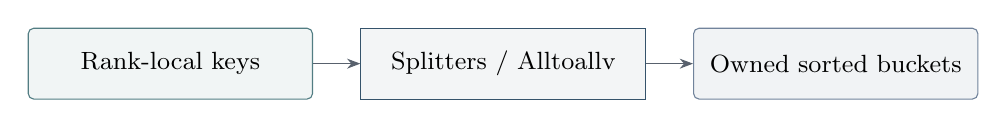
\begin{tikzpicture}[font=\small,>=Stealth,node distance=6mm, every node/.style={align=center,text width=3.4cm,minimum height=9mm,inner sep=3pt}]

\node[draw=cInput,fill=cInput!8,rounded corners=2pt] (a) {Rank-local keys};

\node[draw=cProcess,fill=cProcess!6,right=of a] (b) {Splitters /\allowbreak{} Alltoallv};

\node[draw=cResult,fill=cResult!10,rounded corners=2pt,right=of b] (c) {Owned sorted buckets};

\draw[->,cNeutral] (a)--(b);\draw[->,cNeutral] (b)--(c);\end{tikzpicture}

\caption{Schematic: ownership is separated from the communication or reduction that combines worker results.}\label{fig:flow5}\end{figure}

Rank-local keys -> local sort -> regular samples -> root selects splitters -> broadcast\newline{} Sorted local buckets -> Alltoallv redistribution -> local sort -> distributed global order


Production execution never gathers full input. All runs check local order, consecutive nonempty rank boundaries, element count and two multiset fingerprints. Debug inputs <=\allowbreak{}1 million keys also compare exactly with a gathered serial result. Fingerprints are probabilistic, not proof of exact equality. Serial generation recreates the same p shards; its time excludes generation just as parallel time does.


The measured comparison is shown in Figure~\ref{fig:sort}.

\begin{figure}[htbp]\centering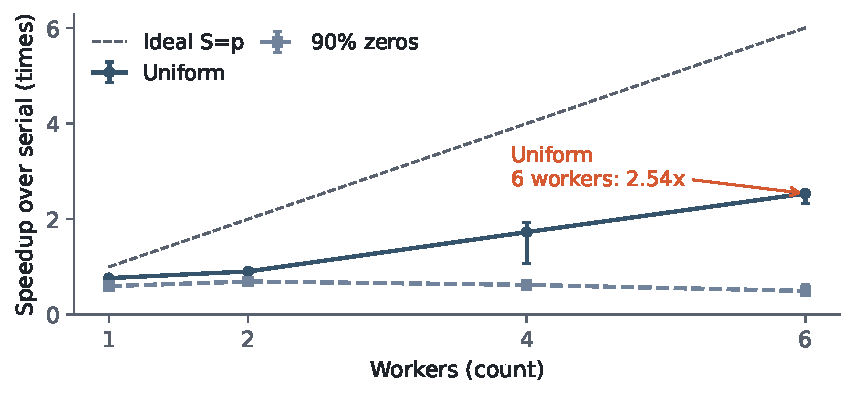
\includegraphics[width=0.9\textwidth]{figures/sort.pdf}

\caption{Duplicate-heavy sample sort scales worse than uniform input: six-rank speedups are 0.50 and 2.54, respectively, for 100 million keys. Points are medians of three runs; whiskers span the minimum and maximum.}\label{fig:sort}\end{figure}

\begin{center}\small\setlength{\tabcolsep}{4pt}\renewcommand{\arraystretch}{1.12}

\begin{tabular}{@{}>{\raggedleft\arraybackslash}p{\dimexpr 0.07955\linewidth-2.545pt\relax}>{\raggedleft\arraybackslash}p{\dimexpr 0.23864\linewidth-7.636pt\relax}>{\raggedleft\arraybackslash}p{\dimexpr 0.25000\linewidth-8.000pt\relax}>{\raggedleft\arraybackslash}p{\dimexpr 0.20455\linewidth-6.545pt\relax}>{\raggedleft\arraybackslash}p{\dimexpr 0.22727\linewidth-7.273pt\relax}@{}}\toprule

\textbf{p} & \textbf{Serial (s)} & \textbf{Parallel (s)} & \textbf{S(p)} & \textbf{E(p)}\\\midrule

1 & 9.002 & 11.76 & 0.7656 & 76.6\%\\

2 & 9.855 & 10.88 & 0.9059 & 45.3\%\\

4 & 9.081 & 5.254 & 1.728 & 43.2\%\\

6 & 9.728 & 3.837 & 2.536 & 42.3\%\\

\bottomrule\end{tabular}\end{center}

Table: uniform keys, oversampling factor one. Each serial baseline is matched to that p-seeded input. Algorithms and size stay fixed, but exact input values vary with p because the assignment asks for per-rank seeds. This is a limitation of strict fixed-dataset strong-scaling interpretation.


\subsection{Critical analysis}

The measured comparison is shown in Figure~\ref{fig:phases}.

\begin{figure}[htbp]\centering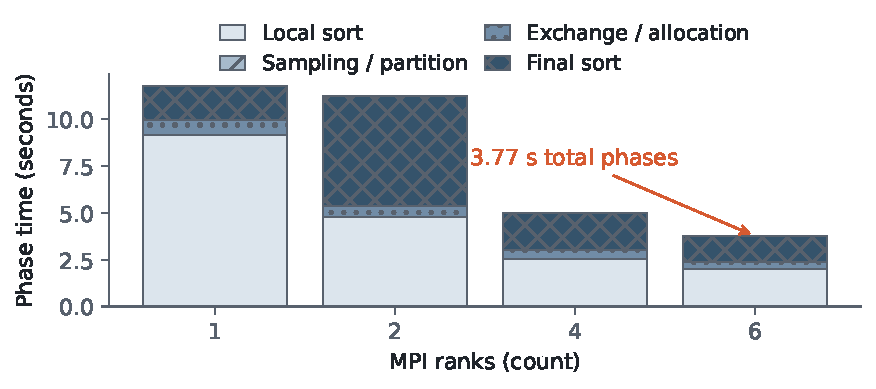
\includegraphics[width=0.9\textwidth]{figures/phases.pdf}

\caption{Uniform sample sort divides its time among local sorting, sampling/\allowbreak{}partitioning, exchange/\allowbreak{}allocation and final sorting. Bars show component medians from three runs on each run's slowest-total rank; they exclude the ending barrier.}\label{fig:phases}\end{figure}

\begin{center}\small\setlength{\tabcolsep}{4pt}\renewcommand{\arraystretch}{1.12}

\begin{tabular}{@{}>{\raggedright\arraybackslash}p{\dimexpr 0.29787\linewidth-4.766pt\relax}>{\raggedleft\arraybackslash}p{\dimexpr 0.21277\linewidth-3.404pt\relax}>{\raggedleft\arraybackslash}p{\dimexpr 0.48936\linewidth-7.830pt\relax}@{}}\toprule

\textbf{Distribution /\allowbreak{} samples} & \textbf{p=\allowbreak{}4 max/\allowbreak{}mean} & \textbf{Final bucket counts}\\\midrule

uniform /\allowbreak{} factor 1 & 1 & 25011792,\allowbreak{}24996146,\allowbreak{}24986646,\allowbreak{}25005416\\

uniform /\allowbreak{} factor 8 & 1.119 & 27981222,\allowbreak{}24001459,\allowbreak{}24011049,\allowbreak{}24006270\\

skew /\allowbreak{} factor 1 & 3.6 & 89996464,0,0,10003536\\

skew /\allowbreak{} factor 8 & 3.6 & 89996464,0,0,10003536\\

\bottomrule\end{tabular}\end{center}

Oversampling changes quantile resolution, but equal splitters still send identical keys to the same bucket. Thus the 90\%-zero input overloads one rank and can leave intermediate ranks empty. More samples cannot fix this partition rule; a secondary global index or explicit equal-key distribution would be required. Correctness checks deliberately skip empty ranks when testing global boundaries.


For uniform data the largest measured phase is local sort at p=\allowbreak{}1 and local sort at p=\allowbreak{}6. Stacks use medians of phases from the slowest-total rank of each run; the sum of component medians need not equal median elapsed time. Ending-barrier wait is excluded from the stack. Exchange includes count transfer and receive allocation as well as Alltoallv.


Ping-pong uses the median zero-byte one-way time for latency alpha=\allowbreak{}2.527e-07 s. Anchoring there, a least-squares fit of median times from 4 KiB through 4 MiB gives beta=\allowbreak{}3.687e-10 s/\allowbreak{}byte and R\textsuperscript{2}=\allowbreak{}0.9917 (three runs/\allowbreak{}size). A balanced p=\allowbreak{}4 model, (p-1)alpha+beta*4N(p-1)/\allowbreak{}p\textsuperscript{2}, predicts 0.02765 s; measured maximum exchange phase is 0.4793 s. This extrapolates beyond calibration messages and compares ideal transfer cost to a wider phase. Shared-memory paths, collective scheduling, bucket imbalance and allocation limit agreement. The unconstrained fitted intercept was -3.85e-05 s; its nonphysical value shows why a single straight-line model across transport regimes needs caution.


Sub-linear speedup is expected: local sorting reduces O(N log N) work per rank, but redistribution still moves O(N) keys, sample selection serializes metadata work, and final local sorting repeats work on received keys. Cache behavior and physical memory bandwidth matter even with perfect buckets. Duplicate-heavy imbalance adds a distinct bottleneck. The implementation supports N<=\allowbreak{}INT\_\allowbreak{}MAX because legacy Alltoallv counts/\allowbreak{}displacements are ints.


\FloatBarrier

\section{Cross-case comparison and reproducibility}

\begin{center}\small\setlength{\tabcolsep}{4pt}\renewcommand{\arraystretch}{1.12}

\begin{tabular}{@{}>{\raggedright\arraybackslash}p{\dimexpr 0.17021\linewidth-5.447pt\relax}>{\raggedright\arraybackslash}p{\dimexpr 0.11702\linewidth-3.745pt\relax}>{\raggedleft\arraybackslash}p{\dimexpr 0.11702\linewidth-3.745pt\relax}>{\raggedleft\arraybackslash}p{\dimexpr 0.12766\linewidth-4.085pt\relax}>{\raggedright\arraybackslash}p{\dimexpr 0.46809\linewidth-14.979pt\relax}@{}}\toprule

\textbf{Case} & \textbf{Model} & \textbf{S(6)} & \textbf{E(6)} & \textbf{Primary costs}\\\midrule

Heat & MPI & 1.029 & 17.2\% & Bandwidth /\allowbreak{} halo synchronization\\

k-mers & OpenMP & 4.085 & 68.1\% & Histogram locality /\allowbreak{} merge traffic\\

Monte Carlo & OpenMP & 6.307 & 105.1\% & Compute /\allowbreak{} runtime overhead\\

PageRank & OpenMP & 1.448 & 24.1\% & Irregularity /\allowbreak{} memory /\allowbreak{} scheduling\\

Sample sort & MPI & 2.536 & 42.3\% & Sorting /\allowbreak{} data redistribution\\

\bottomrule\end{tabular}\end{center}

\textbf{Among the representative six-worker configurations above, Monte Carlo has the highest measured speedup (6.31x).} This compares the listed algorithms and parameters, not universal properties of the domains. Absolute elapsed times, different work sizes and overheads also matter. Poor scaling is an outcome to explain, not a correctness failure.


\subsubsection*{How to reproduce}

In Ubuntu WSL, enter Group04\_\allowbreak{}Assignment3 and run make check. Then run bash tools/\allowbreak{}benchmark.sh on an otherwise idle machine. The script runs sequentially, resumes completed labelled repetitions, and rejects source changes against its SHA-256 manifest. Archive existing results before measuring a different source version or machine. Rebuild before timing; preserve compiler and affinity settings.


Run python tools/\allowbreak{}render\_\allowbreak{}results.py with matplotlib, numpy and reportlab installed to regenerate summary.csv, labelled figures, this report and exactly six PDF slides. The renderer requires three repetitions per group and all planned experiments. Raw results/\allowbreak{}raw.tsv is the source of every performance claim. The sample-sort serial baseline is indexed by both distribution and shard count.


\subsubsection*{Verification and limitations}

The 244 pre-benchmark checks cover uneven heat blocks, one-cell-wide domains, k-mer chunk edges, k=\allowbreak{}1/\allowbreak{}8/\allowbreak{}12, zero-edge PageRank, empty sort ranks, skew, and multiple workers. Invalid argument handling rejects unsupported sizes. Full-scale timing runs disable expensive serial oracles, but sort always checks global order/\allowbreak{}count/\allowbreak{}fingerprints. Version A k-mer races and repeated-stream Monte Carlo are explicitly incorrect demonstrations, never counted as valid speedups.


Measurements were made in WSL on a laptop, not a dedicated cluster. CPU frequency, virtualization, host memory pressure and scheduler interference were not isolated. Only three samples are available at each point. Min-max whiskers show sensitivity; no narrow statistical confidence claim is justified. Profiling hardware counters, memory bandwidth and multi-node MPI would distinguish additional causes. Bonus extensions were not implemented.


\subsubsection*{Artifact map}

\begin{center}\small\setlength{\tabcolsep}{4pt}\renewcommand{\arraystretch}{1.12}

\begin{tabular}{@{}>{\raggedright\arraybackslash}p{\dimexpr 0.40426\linewidth-3.234pt\relax}>{\raggedright\arraybackslash}p{\dimexpr 0.59574\linewidth-4.766pt\relax}@{}}\toprule

\textbf{Artifact} & \textbf{Location}\\\midrule

Buildable implementations & cs1\_\allowbreak{}heat\_\allowbreak{}mpi/\allowbreak{} through cs5\_\allowbreak{}samplesort\_\allowbreak{}mpi/\allowbreak{}\\

Correctness scripts/\allowbreak{}log & tools/\allowbreak{}check*.sh; verification\_\allowbreak{}all.log\\

Raw data /\allowbreak{} summary /\allowbreak{} figures & results/\allowbreak{}raw.tsv; summary.csv; figures/\allowbreak{}\\

Report and six-slide deck & report/\allowbreak{}Group04\_\allowbreak{}report.pdf; slides/\allowbreak{}Group04\_\allowbreak{}slides.pdf\\

Contribution provenance & CONTRIBUTIONS.md; actual member evidence pending\\

\bottomrule\end{tabular}\end{center}

\FloatBarrier

\section{Contributions and references}

\subsubsection*{Individual contributions: awaiting member confirmation}

Actual member hours and authored changes remain unconfirmed. Proposed responsibilities below are not a record of completed work. The consolidated contribution and provenance record is maintained in CONTRIBUTIONS.md. Repository: \href{https://github.com/fatimamalik2307/pdc_assignment3-}{github.com/\allowbreak{}fatimamalik2307/\allowbreak{}pdc\_\allowbreak{}assignment3-}.


\begin{center}\small\setlength{\tabcolsep}{4pt}\renewcommand{\arraystretch}{1.12}

\begin{tabular}{@{}>{\raggedright\arraybackslash}p{\dimexpr 0.25532\linewidth-4.085pt\relax}>{\raggedright\arraybackslash}p{\dimexpr 0.40426\linewidth-6.468pt\relax}>{\raggedright\arraybackslash}p{\dimexpr 0.34043\linewidth-5.447pt\relax}@{}}\toprule

\textbf{Member} & \textbf{Actual hours /\allowbreak{} authored work} & \textbf{Proposed lead /\allowbreak{} reviewer}\\\midrule

Fatima Malik\newline{} 23L-0826 & Not supplied; member confirmation required & Lead 1,3,5; review 2,4\\

Ibrahim Salman\newline{} 23L-0723 & Not supplied; member confirmation required & Lead 2,4; review 1,3,5\\

\bottomrule\end{tabular}\end{center}

The proposed split gives each member at least two leads and two reviews, with neither leading more than three. Final integration, comparison and slides are shared responsibilities. Actual reviews, authored changes, hours and commit records should be recorded as completed. Peer evaluations and presentation rehearsal remain member responsibilities.


\subsubsection*{References}

[1] Supplied course document: \emph{Assignment 3: Parallel Case Studies with OpenMP and MPI}, CS3006, PDC\_\allowbreak{}assignment\_\allowbreak{}3.pdf. Requirements, case definitions and integrity policy; especially Sections 3-7 and 11.


[2] OpenMP Architecture Review Board. \emph{OpenMP API Specification, Version 5.2}. Worksharing, schedules, atomics and reductions. \href{https://www.openmp.org/spec-html/5.2/openmp.html}{openmp.org/\allowbreak{}spec-html/\allowbreak{}5.2/\allowbreak{}openmp.html}. Accessed 23 November 2026.


[3] Open MPI. \emph{Version 4.1 documentation}. Cartesian topology, point-to-point requests and collectives. \href{https://www.open-mpi.org/doc/v4.1/}{open-mpi.org/\allowbreak{}doc/\allowbreak{}v4.1/\allowbreak{}}. Installed runtime: 4.1.6. Accessed 23 November 2026.


[4] D. Chakrabarti, Y. Zhan and C. Faloutsos. \emph{R-MAT: A Recursive Model for Graph Mining}. SIAM International Conference on Data Mining, 2004, pp. 442-446. \href{https://doi.org/10.1137/1.9781611972740.43}{doi:10.1137/\allowbreak{}1.9781611972740.43}. Synthetic graph method; no external dataset was downloaded.


[5] Reproducibility evidence generated with this package: results/\allowbreak{}raw.tsv, environment.txt, host\_\allowbreak{}machine.json, sources.sha256, pingpong\_\allowbreak{}1.csv through pingpong\_\allowbreak{}3.csv, and verification\_\allowbreak{}all.log. These are the primary sources for all numerical claims in the report.


\subsubsection*{Project records}

The package includes code, measured graphs, this report, six slides and a ZIP. CONTRIBUTIONS.md is the source of the provenance disclosure and contribution status; GIT\_\allowbreak{}COMMIT\_\allowbreak{}PLAN.md records the proposed import sequence. Performance claims are supported by the retained measurement data.


\FloatBarrier\end{document}